%
%
%
\section{Interpretation}%
  %
  %
  \label{sec:linreg}
  %
  %
  \index{Linear regression!Interpretation}%
  %
  %

We will use a breakdown of Table~\ref{tbl:hibbs_yx1_regress} to explain standard Stata output for the \cmd{reg} command, which estimates the simple linear regression model \texttt{reg bread vote}. You should read your model by looking briefly at the \emph{goodness of fit} of the model, and then focus on understanding the \emph{regression coefficients}.

% \begin{table}[htp]
% 	\begin{itemize}
% 		\item \emph{Analysis of variance} (left) and \emph{goodness of fit} (right):\\
% 		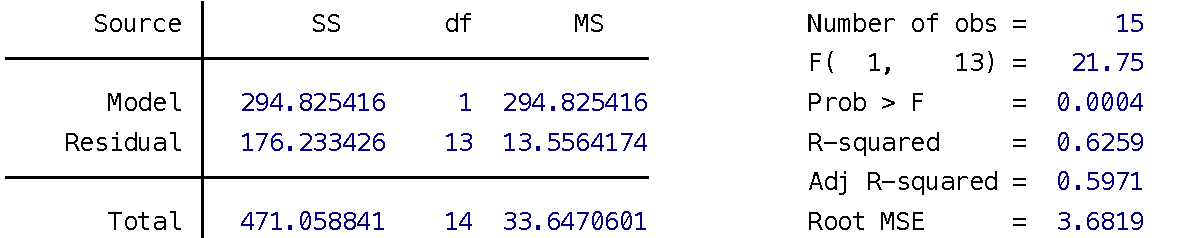
\includegraphics[scale=.5]{images/hibbs_yx1_regress_top.pdf}
% 	
% 		\item \emph{Regression coefficients}, including constant (\texttt{\_cons}):\\
% 		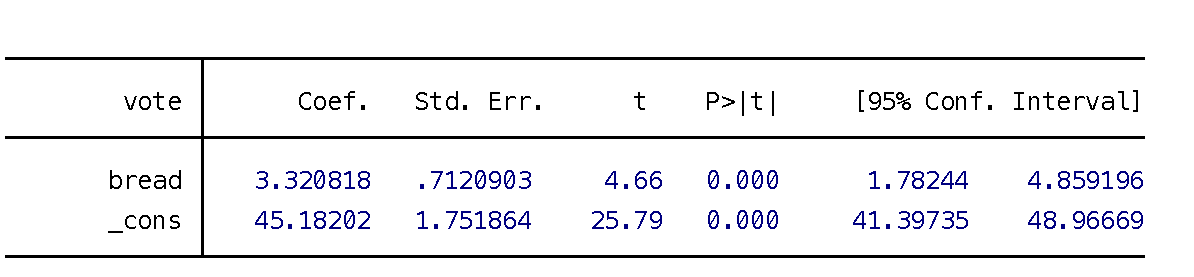
\includegraphics[scale=.5]{images/hibbs_yx1_regress_bottom.pdf}
% 	\end{itemize}
% 
% 	\caption[Breakdown of regression output with \cmd{reg}]{\label{tbl:hibbs_yx1_regbits}
% 	Breakdown of regression output with \cmd{reg}.\\
% 	\hibbs}
% \end{table}%

	%
	% 6.1.1
	%
	\subsection{Goodness of fit}%
    \index{Linear regression!Goodness of fit}%
    \label{sec:goodness}%
	%
	Table~\ref{tbl:regression_fit} shows the variance table (left), which details the sum of squares for the model and for its residuals. This information is redundant with an analysis of variance, and is used to derive information on the goodness of fit (right):

	\begin{table}[htp]
		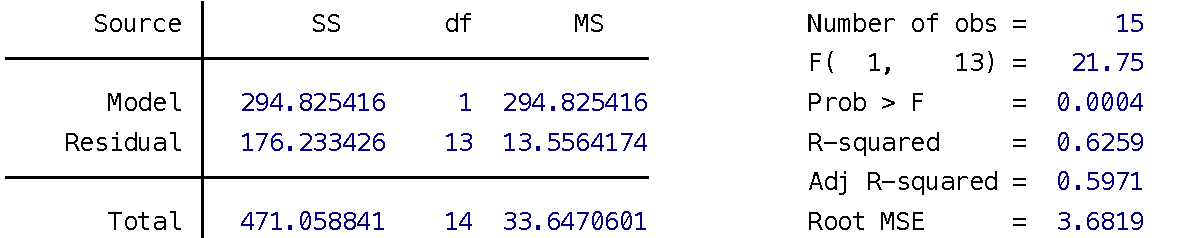
\includegraphics[scale=.5]{images/hibbs_yx1_regress_top.pdf}

	  	\caption[Extract from \cmd{reg} output (1): Variance and goodness of fit]{\label{tbl:regression_fit}%
		Extract from \cmd{reg} output (1): %
    Variance and goodness of fit. %
		\hibbs}
	\end{table}%

	\begin{itemize}
		\item The \textbf{number of observations} constrains your whole model: all statistical results are derived from and only from the set of observations included in the linear regression, after listwise deletion (explained on p.~\pageref{casewise}). The model cannot be more intelligent than this set of observation: only you can. If a large fraction of the data is not represented in the analysis, you will have to describe the subset on which you are running your analysis, and assess to what extent you can generalize its results.

		\item The \textbf{$F$-statistic} is used to test whether your model is significantly different from the null estimator $H_0: \beta = 0 \Rightarrow \beta X = 0 \Rightarrow Y = \alpha$. In other words, it tests whether the regression line of your model is `flat' and equivalent to the mean value of $Y$ in its ability to describe its distribution. This is the null hypothesis of regression overall, and is also used for each coefficient in the model. The substantive significance of your model will rarely need to verify this hypothesis.\footnote{This means that, in theory, there is no real grounds to be concerned about the $p$-value of the $F$-test. What happens in practice is that multiple regression models quickly become statistically significant.}
		
		\item The \textbf{$R^2$ (R-squared)} is the ratio of predicted variance, $\sum{(\hat{Y_i}-\bar{Y_i})^2}$, by the total variance in the data, $\sum{(Y_i-\bar{Y_i})^2}$, for $i=1, \ldots, n$ observations. As the unpredicted variance (RSS) approaches 0, the $R^2$ will approach 1, which makes it simple to understand. The adjusted $R^2$ corrects for factors that artificially inflate the statistic.\footnote{There is a wealth of other measures that penalize even more the predicted variance, to obtain more conservative estimates of how much is actually predicted. For social science data, this game is generally not so relevant.} In the present example, the `Bread and Peace' model therefore predicts around 60\% of the variance in presidential votes on 15 postwar elections, which is statistically remarkable.
		
		The substantive significance of the $R^2$ is limited: it is perfectly justifiable to research an association that does not efficiently minimizes unpredicted variance. You should, however, use it to compare the predictive exhaustiveness of several models. Table~\ref{tbl:hibbs_yx1_estout} provided an example of such a comparison: the `Bread and Peace' model, which is already highly efficient over all election years ($R^2\approx.6$), can become even more efficient without election years affected by war ($R^2\approx.8$). In a multiple regression, you might also want to try out several models to compare how much your model changes in absence or presence of a single variable.

		% http://www.theanalysisfactor.com/small-r-squared/

		\item\label{rmse_explained} The \textbf{Root MSE} (Root Mean Square Error) is the RMSE briefly mentioned at p.~\pageref{rmse}, and is another way to understand the error term of the model. The RMSE is measured in the same units as the dependent variable $Y$ and indicates the mean distance between fitted and actual data points. In the present example, the `Bread and Peace' model is therefore, on average, three percentage points wrong about the actual presidential vote. This measure is meaningful only if you can interpret it: in the case of a presidential election, three percentage points is a meaningful margin of error.

	\end{itemize}

	%
	% 6.1.2
	%
  % unstd, std, dummies
  %
	\subsection{Regression coefficients}%
    \index{Linear regression!Regression coefficients}%
    \index{Regression models!Coefficients!Linear regression}%

	\paragraph{Interpreting coefficients}%
  	\label{sec:coefficients}%
	%
	Table~\ref{tbl:regression_coef} shows the regression coefficients and related information, which is the heart of the model. Whether your model is statistically significant or whether it captures a large fraction of variance is of limited importance in comparison to the coefficient estimates of the regressors. A statistically insignificant model, for instance, will fail to estimate a single reliable predictor. In practical terms, this implies you need not spend more than a minute on the goodness of fit of your model, and should instead pay \emph{more than careful} attention to its coefficients:

	\begin{table}[htp]
		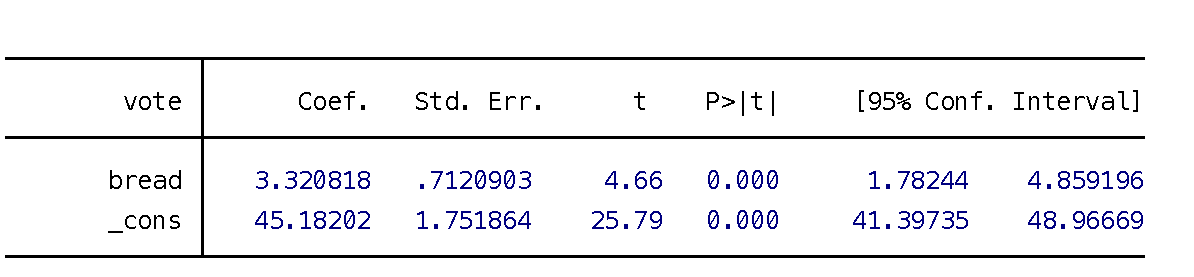
\includegraphics[scale=.5]{images/hibbs_yx1_regress_bottom.pdf}

	  	\caption[Extract from \cmd{reg} output (2): Regression coefficients]{\label{tbl:regression_coef}%
        Extract from \cmd{reg} output (2): %
        Regression coefficients. %
		    \hibbs}
	\end{table}%

	The coefficients, or regression \emph{parameters}, were estimated through \emph{maximum likelihood}\index{Models!Maximum Likelihood Estimation (MLE)}, a method of estimation that can be used with several regression models.\footnote{Maximum likelihood estimation (MLE) is also used for logistic regression, which is briefly described and illustrated at p.~\pageref{ch:log}.} What they intend to measure, beyond the statistical significance of the independent variable $X$ for predicting the dependent variable $Y$, is its \emph{marginal effect}\index{Linear regression!Marginal effects}\index{Marginal effects|seealso{Linear regression}}: as in the linear function $Y=\beta X$, when $X$ increases by one unit, $Y$ increases by $\beta$ units, where $\beta$ is the regression coefficient of $X$. If the coefficient is negative, then $Y$ decreases by $\beta$ units when $X$ increases by one unit.

	In the present example, the model `starts' at the constant, $\alpha \approx 45.18$, which is the level of presidential support $\bar Y$ predicted by the model when the \texttt{bread} parameter is null (or, in quick notation, $\alpha = E(Y|X=0)$). This constant is theoretical and not always as meaningful as it is here. This is because from that point, the model predicts that every increase in one unit of the \texttt{bread} variable (real growth in disposable income, in \%) is associated to an increase in $\beta \approx 3.32$. Linear regression is an additive model, and the regression parameter is positive, which is why it makes sense to describe the model as an engine that estimates `constant' presidential support around 45\%, and then predicts a `marginal' increase of 3.3 percentage points in support for each percentage point of real disposable income growth.
	
	Table~\ref{tbl:hibbs_yx1x2} illustrates how this rule of calculation stays true when you add variables to perform \emph{multiple linear regression}. Regression coefficients are estimated for each variable while holding all other variables constant at zero value. For that reason, they are ceteris paribus measures that capture the effect of each variable ``all things equal'' \ie all other model variables held at a constant value of nil. In our example, the addition of the \texttt{death} variable to the model shows that every U.S. fatality per million population reduces presidential support by $\beta_2 X_2=-.05$. This effect is a `net' effect, \emph{independent} of the economic circumstances captured by the \texttt{bread} variable. In parallel, the positive effect of income growth on presidential support is verified while \emph{controlling for} the effect of military fatalities.

	\begin{table}[htp]
		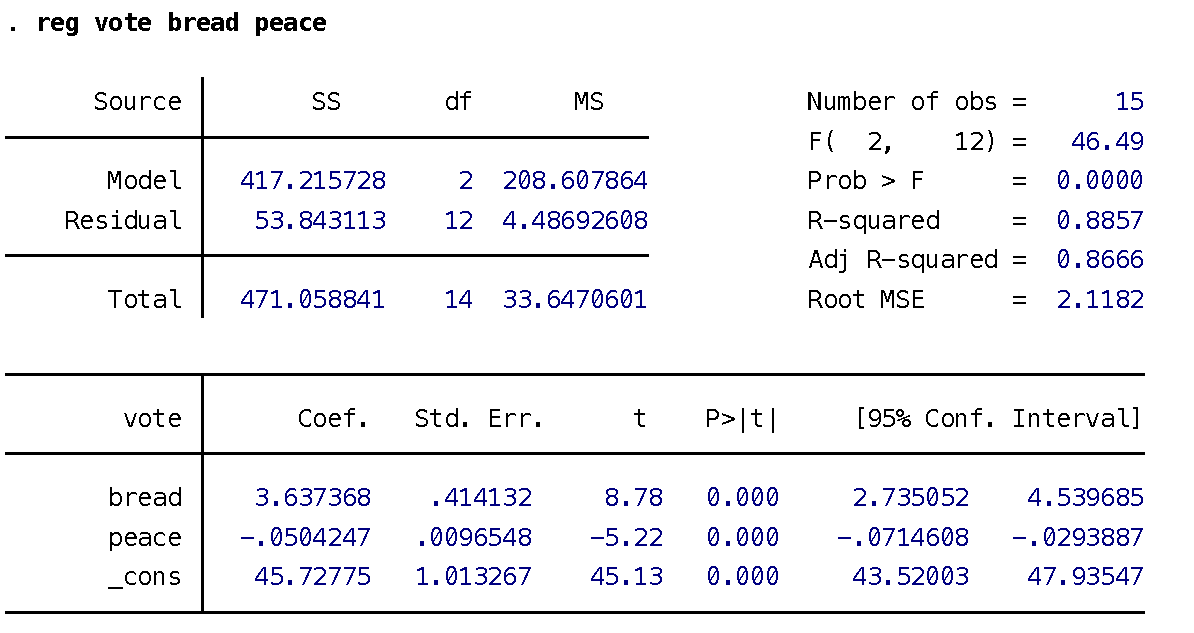
\includegraphics[scale=.5]{images/hibbs_yx1x2.pdf}

	  	\caption[Extract from \cmd{reg} output (3): %
        Multiple regression coefficients]{\label{tbl:hibbs_yx1x2}%
		    Extract from \cmd{reg} output (3): %
        Multiple regression coefficients. %
        \hibbs}
	\end{table}%
	
	Any model that yields one statistically significant coefficient can be interesting to interpret, but make sure that you read regression coefficients within their confidence bounds: standard errors can be quite large in low-$N$ samples, and their confidence intervals can be consequently large too, as is the case here in the `Bread and Peace' model. Stata displays the standard errors and the ratio between the coefficient and its standard error, the $t$-value, which is used to compute the $p$-value from the $t$-distribution. If the confidence interval of your coefficient comes close to include zero, then its marginal effect might well be null or close to null.
	
	To assess whether you know enough about the coefficients of your model, try fitting a real value of $Y$. For example, in the simplified `Bread and Peace' model that is presented here, a stable income growth of $X_1=2$ percentage points with a low number of $X_2=50$ war casualties per million population leads to a predicted electoral support of $\hat Y = 45.7 + 2*3.6 + 50*(-.05) \approx 50.4\%$ in favor of the incumbent president.

	\paragraph{Dummies}%
	\label{sec:dummies}%
	%
	Dummies are a way to measure a dichotomous condition, such as being female (1) or non-female (0), White (1) or non-White (0), etc. The parametric estimate of a dummy variable is the independent effect of that condition when it is verified in the data. In the regression equation, a dummy is just a true/false condition for a coefficient, as in this example equation that compares the value of a dependent variable $Y$ in democracies versus dictatorships:

	\[
	  Y = \alpha + \beta_1 X_1 + \beta_2 X_2 + {\color{red}\beta_3 \times \text{democracy}} \left\{ 
	  \begin{array}{l l}
	    \text{if~democracy}=0 \\ \quad Y = \alpha + \beta_1 X_1 + \beta_2 X_2 + \beta_3 \times 0\\[1em]
	    \text{if~democracy}=1 \\ \quad Y = \alpha + \beta_1 X_1 + \beta_2 X_2 + \color{red}\beta_3 \times 1\\
	  \end{array}\right\}
	\]
	
	In this equation, the \texttt{democracy} coefficient is not estimated for dictatorships, which means that the dictatorship category is the \emph{reference category}, or the \emph{baseline} of your model. The \texttt{democracy} coefficient $\beta 3$ in the regression represents the \emph{net effect} on this baseline. You can code any categorical variable as one or more dummies with either \cmd{recode} or \cmd{tab}{tabulate} with the \texttt{gen(dummy)} option, and therefore calculate the net effect of each categorical predictor.

	Table~\ref{tbl:abortion_dummy} shows a practical example of a dummy coding for democratic regimes in a multiple linear regression at the country level. The dummy is preceded by the \cmd{i.}{interaction} prefix command. The coefficient for the \texttt{1.democracy} variable indicates how the dependent variable compares in democracies versus dictatorships when holding all other variables in the model constant. The coefficient is positive, indicating that on average, democracies enjoy higher support for abortion; the standard error on that estimate, however, is too high, and the coefficient is statistically insignificant.

	In that same regression table, another categorical variable codes for political regime: \texttt{dpi\_system} distinguishes presidential, parliamentary and mixed regimes. In the \texttt{dpi\_system} variable, presidential regimes were coded \texttt{0} and are the reference category. The overall model therefore uses dictatorial presidential regimes to measure whether support for abortion is higher or lower in other regimes, the results of which are the dummy coefficients. In this example, the only statistically significant category codes for parliamentary regimes (\texttt{dpi\_system~==~2}).

	\begin{table}[htp]
		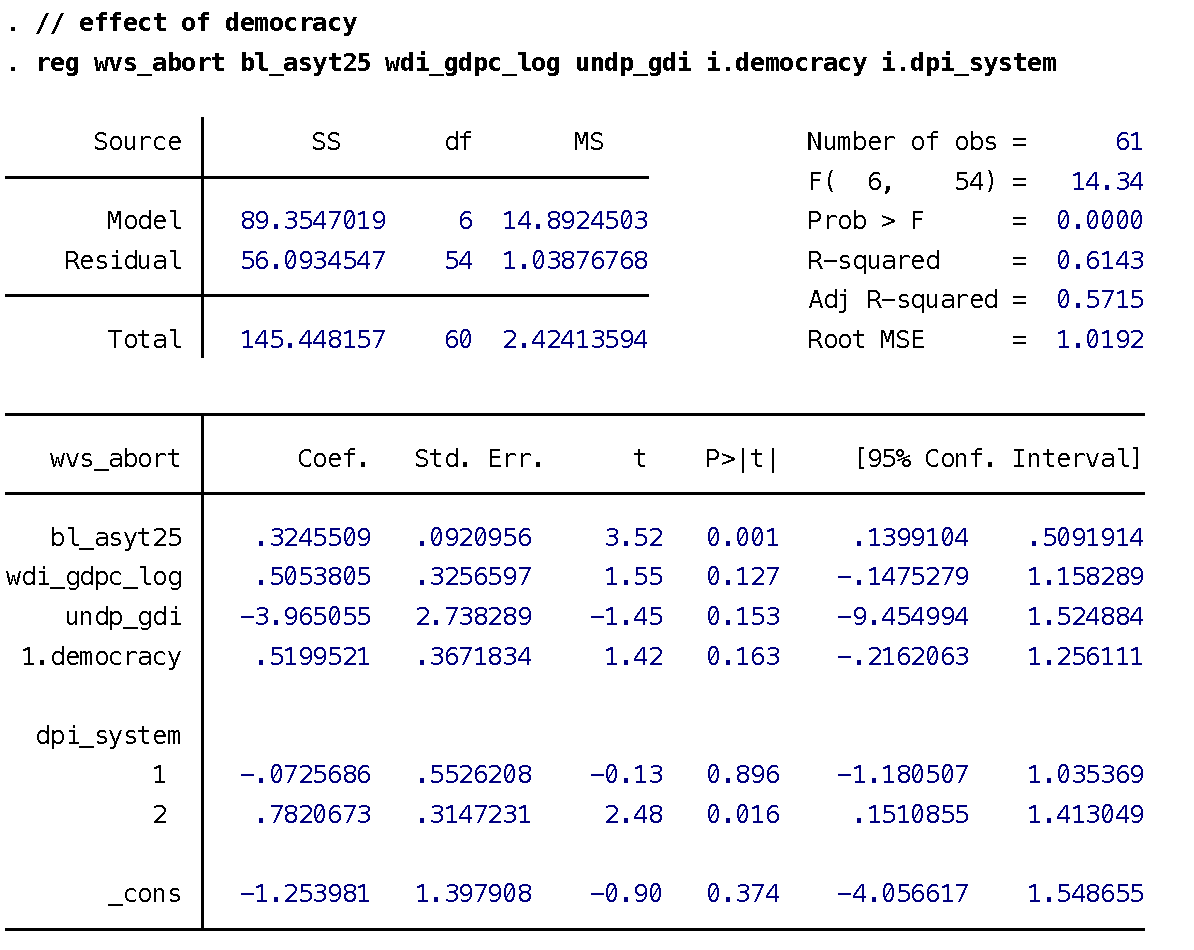
\includegraphics[scale=.5]{images/abortion_dummy.pdf}

	  	\caption[Linear regression with a dummy]{\label{tbl:abortion_dummy}%
        Linear regression with the \texttt{i.democracy} dummy, %
        recoded from variable \texttt{gol\_polreg}. %
		    \qog}
	\end{table}%
	
	Figure~\ref{fig:abortion_dummy_plot} shows how this dummy translates graphically: democracies and dictatorships have been estimated in the same way, using the same variables with the same coefficients. However, the regression line for democracies (red) is slightly above the baseline model for dictatorships (blue). The distance between the two parallel regression lines is the (positive) net effect of \texttt{i.democracy} on the dependent variable \texttt{wvs\_abort}. This effect is rather minor, since many other predictors are also correlated to democracy and absorb most of its variance.

	\begin{figure}[htp]
		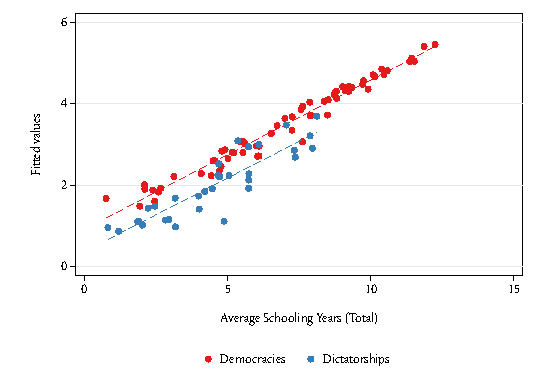
\includegraphics[width=.9\textwidth]{images/abortion_dummy_plot.pdf}

		\caption[Plotting the effect of a dummy]{\label{fig:abortion_dummy_plot}%
		Plotting the effect of the \texttt{i.democracy} dummy with two linear fits of Table~\ref{tbl:abortion_dummy}. %
		\qog}
	\end{figure}%

	Stata will accept the \cmd{i.}{interaction} prefix command in front of any categorical variable, and will select the first category as the baseline. Dummies are simple to implement but are useful \emph{only once you know the baseline of the model}. If you are coding a lot of information as dummies, then your model describes a theoretical `zero' situation where all dummies are equal to nil. Since you have to interpret dummies in reference to that situation, make sure that you understand what is the reference category of each dummy.

	% http://www.theanalysisfactor.com/confusing-statistical-term-6-factor/
  
	\paragraph{Standardized coefficients with \opt{beta}{regress}}%
	\label{sec:beta}%
	%
	Your coefficients can be interpreted in more than metric form. It might well be, for instance, that your variables have been transformed in such as way, or measured in such units, that metric coefficients will make little sense even when statistically significant. The fundamental problem lies with the units of your coefficients, which are dependent on the units of measurement of your variables. For example, given that education and income have different units, you cannot compare the effect of education (which the coefficient measures in years of schooling) and income (which the coefficient measures in constant dollars). Identically, the `Bread' and `Peace' variables are calculated on different units of different distributions.
	
	Table~\ref{tbl:hibbs_yx1x2_beta} shows how to solve that issue with standardized, a.k.a `beta' coefficients. These coefficients are measured from a standardized measure of each $Y$ and $X$ variable, and therefore share the same units. When you add the \opt{beta}{regress} option to the \cmd{reg} command, these coefficients replace the confidence intervals in the Stata output.

	\begin{table}[htp]
		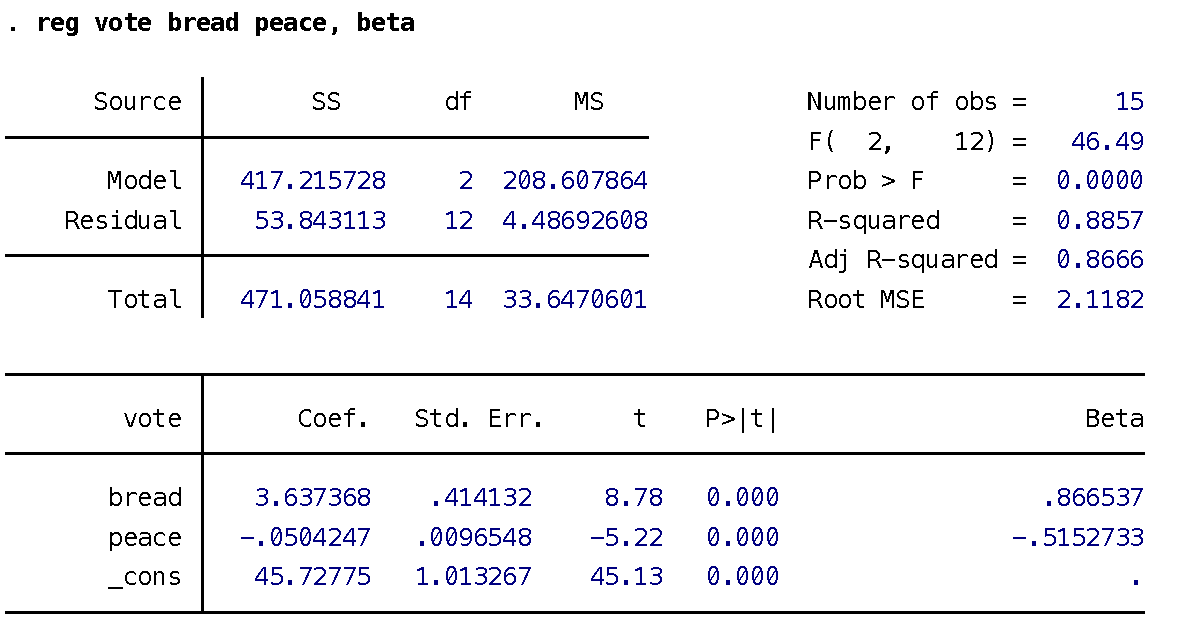
\includegraphics[scale=.5]{images/hibbs_yx1x2_beta.pdf}

	  	\caption[Extract from \cmd{reg} output (5): Standardized regression coefficients]{\label{tbl:hibbs_yx1x2_beta}%
      Extract from \cmd{reg} output (5): Standardized regression coefficients. %
      \hibbs}
	\end{table}%
	
	Standardized coefficients should be read as an approximate measure of \emph{statistical} influence: the more variance a variable captures, the further away from zero its standardized coefficient will be. The positive or negative sign does not apply to the magnitude of standardized coefficients, only their `distance' to zero. This is not a measure of substantive influence or even less causal influence by any means. However, it gives you a hierarchy of importance that shows, for example, that the `Bread and Peace' model is primordially driven by the \texttt{bread} (economy) variable, whose standard coefficient is close to .8, while the peace variable carries less statistical weight with an \emph{absolute} standardized coefficient of .51.
  
	%
	% 6.1.3
	%
	\subsection{Exporting results}

  % leanout
  % estout
  % plotbeta (?)

\paragraph{Exporting with \cmd{estout}}%
  \index{Linear regression!Storing estimates}%

Table~\ref{tbl:hibbs_yx1_estout}, finally, shows a few more commands to format your results straight away for storage and export with the \cmd{estout} package. The \cmd{eststo} command stores the estimates of any number of models, and the \cmd{esttab} command allows selecting only part of the regression output, for viewing and/or exporting purposes.

\begin{table}[htp]
	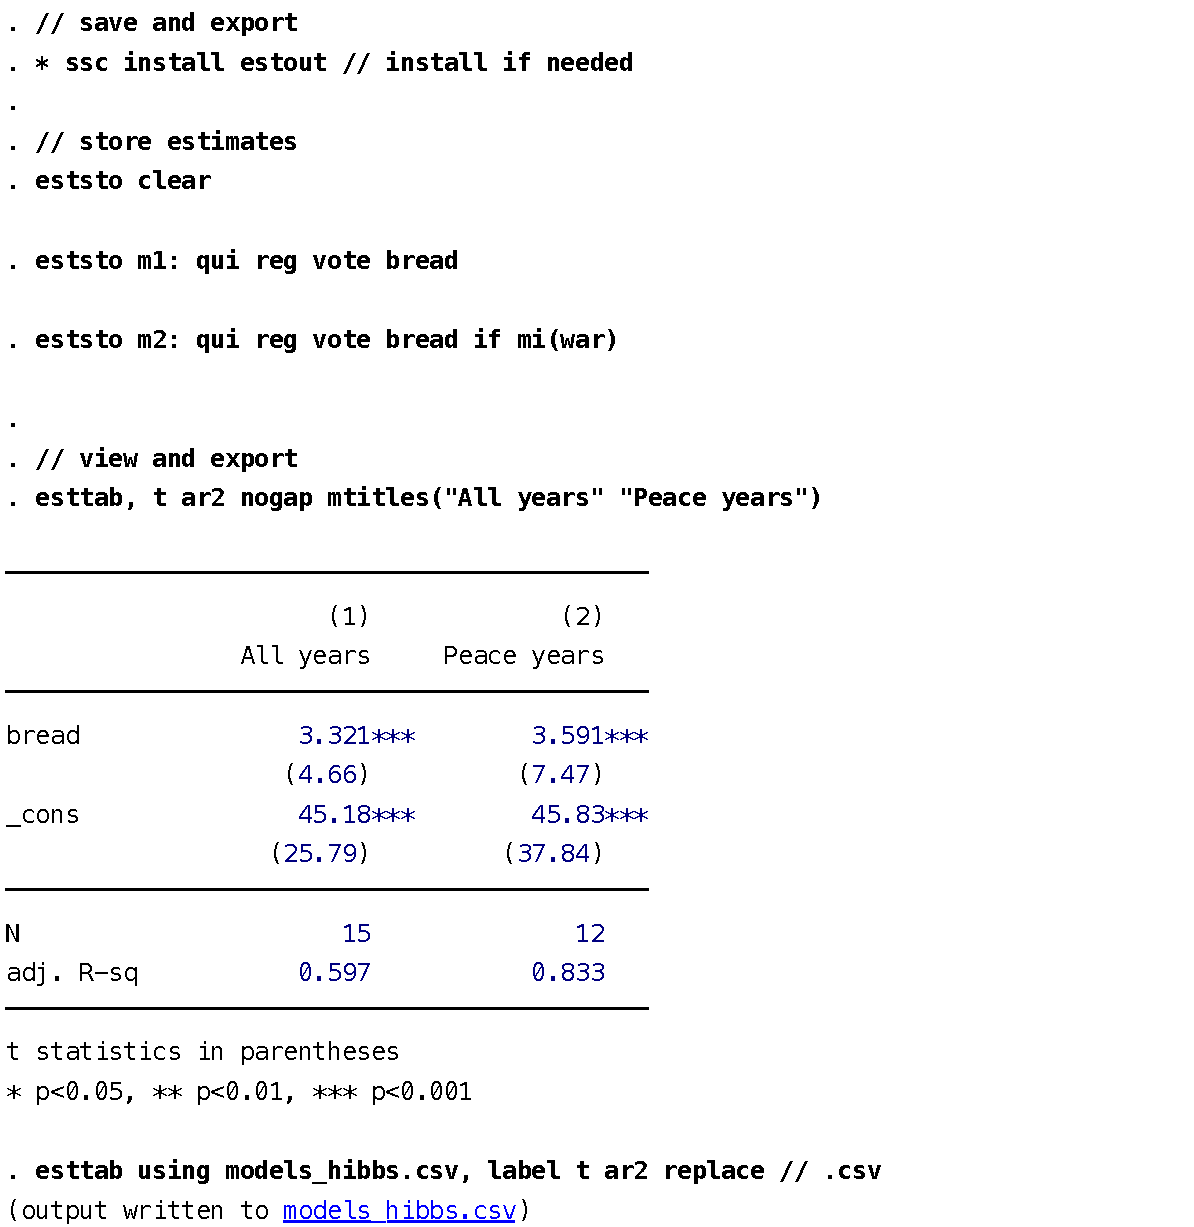
\includegraphics[scale=.5]{images/hibbs_yx1_estout.pdf}

	\caption[Storing estimates with \cmd{predict}]{\label{tbl:hibbs_yx1_estout}%
    Storing and exporting estimates with \cmd{estout}. %
	  See \statacode{help estout} and related online documentation for options. %
    \emph{Note:} the \cmd{reg} command is muted by the \cmd{qui}{quietly} command in this code; %
    its output does not show up on screen, but the command ran `silently' in the background. %
    \hibbs}
\end{table}%

\paragraph{Formatting instructions}

%
%
%
\index{Linear regression!Exporting results}
\paragraph{Regression estimates}

Table~\ref{tbl:hibbs_yx1_predict} shows how to pass several \cmd{predict} commands to store some estimates. We store the fitted values under the name \texttt{yhat} in reference to $\hat{Y}$, the estimated values of the dependent variable $Y$: for every $i=1, \ldots, n$ observations, $Y_i = \hat{Y_i} + \epsilon_i$. To store the residuals in the units of the dependent variable, we use \cmd{predict} with the \coab{resid}{residuals}{predict} option. The standardized residuals, calculated in standard deviations of their own distribution, are stored with the \coab{rsta}{rstandard}{predict} option.

\begin{table}[htp]
	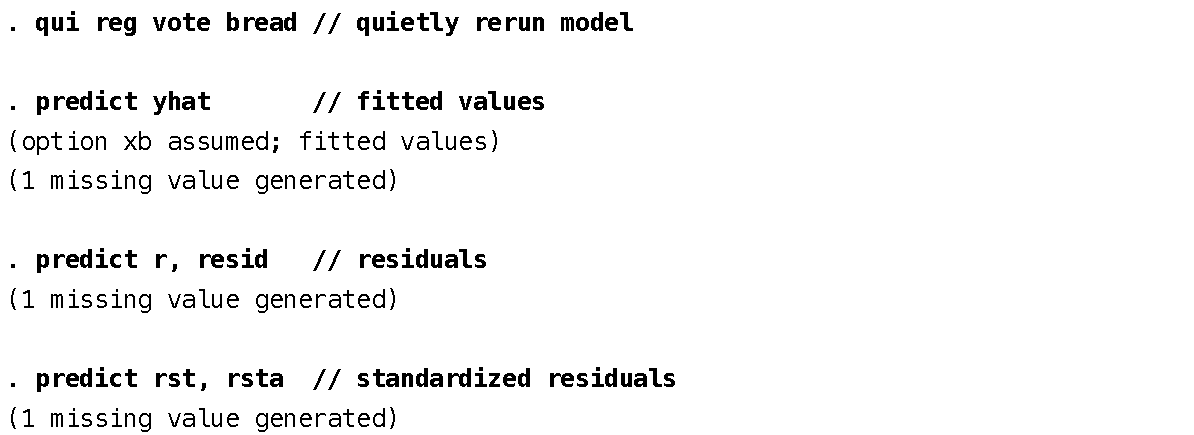
\includegraphics[scale=.5]{images/hibbs_yx1_predict.pdf}

	\caption[Storing estimates with \cmd{predict}]{\label{tbl:hibbs_yx1_predict}%
	Storing estimates with \cmd{predict}. %
	\hibbs}
\end{table}%

Prior to interpreting the content of the regression table/output, a good idea is to take care of saving the model results straight away, in simplified format.

Table~\ref{tbl:estout_reg} shows regression output exported with \cmd{estout} as shown at p.~\pageref{tbl:hibbs_yx1_estout}. Models are each in a separate column with a short title, and a lot of information has been dropped to reflect the most relevant aspects of the model. If you need more sophisticated output, Ben Jann's online documentation for \cmd{estout} contains useful examples.%
\footnote{\url{http://repec.org/bocode/e/estout/index.html}.}

% If you are focusing on standardized coefficients, you can produce an even more simplified output with the \opt{beta}{esttab} and \texttt{not} options.

\begin{fullwidth}
	\begin{table}
		\footnotesize
    %
    {
\def\sym#1{\ifmmode^{#1}\else\(^{#1}\)\fi}
\begin{tabular}{l*{4}{c}}
\hline\hline
                    &\multicolumn{1}{c}{(1)}&\multicolumn{1}{c}{(2)}&\multicolumn{1}{c}{(3)}&\multicolumn{1}{c}{(4)}\\
                    &\multicolumn{1}{c}{Full model}&\multicolumn{1}{c}{Controls}&\multicolumn{1}{c}{Theocracy}&\multicolumn{1}{c}{GII}\\
\hline
No Schooling, Female and Male (25+)&         0.0         &        -0.0         &         0.0         &         0.0         \\
                    &       (0.0)         &       (0.0)         &       (0.0)         &       (0.0)         \\
[1em]
Log(Population)     &        -0.1         &        -0.2         &        -0.1         &        -0.1         \\
                    &       (0.1)         &       (0.1)         &       (0.1)         &       (0.1)         \\
[1em]
Log(GDP per capita) &         0.3         &         1.0\sym{***}&         0.2         &         0.4         \\
                    &       (0.3)         &       (0.2)         &       (0.2)         &       (0.3)         \\
[1em]
c.undp\_gii#c.wvs\_theo&       -10.2\sym{**} &                     &                     &                     \\
                    &       (3.0)         &                     &                     &                     \\
[1em]
Support for theocracy&                     &                     &       -10.5\sym{***}&                     \\
                    &                     &                     &       (1.7)         &                     \\
[1em]
Gender Inequality Index&                     &                     &                     &        -4.8\sym{**} \\
                    &                     &                     &                     &       (1.6)         \\
[1em]
Constant            &         4.4         &        -1.7         &         8.6\sym{**} &         3.3         \\
                    &       (3.3)         &       (3.1)         &       (2.7)         &       (3.4)         \\
\hline
Observations        &          41         &          49         &          42         &          48         \\
rmse                &         1.0         &         1.2         &         0.8         &         1.1         \\
\hline\hline
\multicolumn{5}{l}{\footnotesize Standard errors in parentheses}\\
\multicolumn{5}{l}{\footnotesize \sym{*} \(p<0.05\), \sym{**} \(p<0.01\), \sym{***} \(p<0.001\)}\\
\end{tabular}
}

		%
		\caption{Regression output produced with \cmd{estout}.}
		\label{tbl:estout_reg}
	\end{table}
\end{fullwidth}

To produce this example, we first stored some example specifications of a linear regression model into short names \texttt{m1} to \texttt{m4}. To store a model, simply prefix its command with \texttt{eststo (name): qui}, which will quietly run the model and save it under \texttt{(name)}:

\begin{docspec}
  * example data\\%
  use bl\_lu\_25mf undp\_gii wvs\_abort wvs\_theo unna\_pop wdi\_gdpc using data/qog2013, clear\\%
  * log-transformations\\%
  gen log\_pop = ln(unna\_pop)\\%
  la var log\_pop "Log(Population)"\\%
  gen log\_gdpc = ln(wdi\_gdpc)\\%
  la var log\_gdpc "Log(GDP per capita)"
  %% block above repeated from session 5, choose onyl one destination
  * example models\\%
  eststo m1: qui reg wvs\_abort bl\_lu\_25mf log\_* c.undp\_gii\#c.wvs\_theo\\%
  eststo m2: qui reg wvs\_abort bl\_lu\_25mf log\_*\\%
  eststo m3: qui reg wvs\_abort bl\_lu\_25mf log\_* wvs\_theo\\%
  eststo m4: qui reg wvs\_abort bl\_lu\_25mf log\_* undp\_gii
\end{docspec}

Note that the full model has an interaction term, and that the three other models simply show how the model behaves under slightly different specifications. The entire output is exported with a single command, \cmd{esstab}:

\begin{docspec}
  * export regression output with -estout-\\%
  esttab m1 m2 m3 m4 using models.csv, ///\\%
    replace label b(1) se(1) sca(rmse) ///\\%
  	mti("Full model" "Controls" "Theocracy" "GII")
\end{docspec}

The \texttt{b(1)} and \texttt{se(1)} options set the unstandardised coefficients and standard errors to one digit precision. The \texttt{sca(rmse)} option adds the RMSE to each model, for which names are set by the \texttt{mti} option.

The \cmd{estout} package is very flexible. The example shown uses only $t$-statistics (option \texttt{t}) and adjusted $R^2$ (option \texttt{ar2}), but you can cook different output with standard errors (option \texttt{se}) and standardized coefficients (option \opt{beta}{esttab}), depending on your preferred method of reading. The next section explains how each of these elements inform the model.

Finally, note that the code used with the \cmd{estout} command actually estimates \emph{two} models: `Model 1' was estimated on all elections years ($N=15$), while `Model 2' was estimated only on $N=12$ elections years for which military fatalities were not a significant factor. The estimates can be compared between models, which we will also illustrate below.

	
	\paragraph{Simplifying interpretation with \cmd{leanout}}%
	\label{sec:leanout}
	%
	The \cmd{leanout} package is a prefix command that reduces regression output to a minimum, so that you can concentrate on the essentials. The \texttt{estout} package already introduced that logic: Table~\ref{tbl:hibbs_yx1_estout} at p.~\pageref{tbl:hibbs_yx1_estout} showed only a few statistics in comparison to the standard Stata output, with much less precision to better represent the true level of accuracy in social science data. The output of the \cmd{leanout} command is also ``rather draconian'' and loses all information related to the $t$-tests, focusing instead on the actual values of the coefficients and their standard errors.\footcite{Beck:2010}

	Table~\ref{tbl:hibbs_yx1x2_leanout} shows \cmd{leanout} syntax and output. Again like \cmd{estout} command, the \cmd{leanout} command is a prefix to the \texttt{reg} command (and to other regression commands).
	
	\begin{table}[htp]
		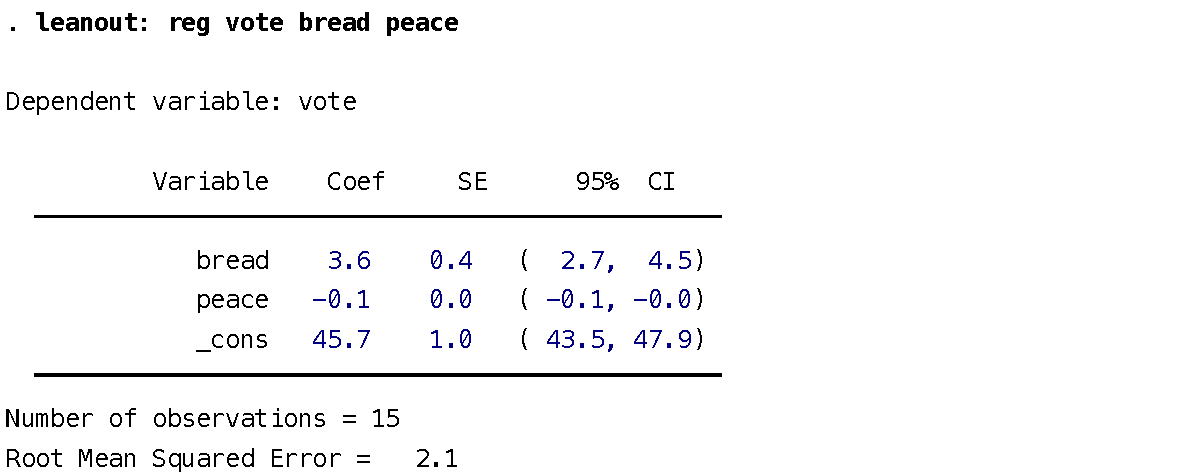
\includegraphics[scale=.5]{images/hibbs_yx1x2_leanout.pdf}

	  	\caption[Extract from \cmd{reg} output (4): Simplified regression output]{\label{tbl:hibbs_yx1x2_leanout}%
      Extract from \cmd{reg} output (4): %
      Simplified regression output using the \cmd{leanout} prefix. %
      \hibbs}
	\end{table}%
	
	The drastic reduction of information obtained through \cmd{leanout} is a good exercise in itself to check whether you understand regression coefficients correctly. The parameters selected by \cmd{leanout} are expressed in real-world units, which encourages the reader to read standard errors, confidence intervals and the RMSE rather than $p$-values. This approach makes sense, especially when interpreting unstandardized coefficients for untransformed variables, because in that case, you are able to read coefficients in the same metric as the actual variables, such as years, currencies, percentage points or counts (\ie numbers of something: alcoholic beverages per week, sexual partners in the last five years, whatever).

	%If you find it difficult to interpret coefficients without their significance tests with $t$-values and $p$-values, then you are experiencing exactly what any conventional quantitative social researcher would experience in the same situation.
	Frequentist statistics, like linear regression analysis, insist heavily on measuring the probability level of the null hypothesis. The interpretation of $p$-values, however, is substantively limited: a $p$-value does not indicate the strength of an association, and it does not translate as the chance of a significant association.\footnote{Even when Stata displays a probability level as `\texttt{Pr = 0.000},' it really means that $p < .0001$.}
	
	If you are on your way to analyze the data \emph{metrically}, which is a best-case scenario, then \cmd{leanout} will force you to consider the confidence bounds of your parameters and the proximity of the whole confidence interval to zero. In absence of a `star system' and $p$-values, you are also forced to consider the actual value of the standard errors. Intellectually, the end process is equivalent to forming an opinion about music without being influenced by a music market where media charts and corporate promotion end up excessively shaping your tastes.
	
	The overall aim of minoring $p$-values is to increase freedom in probabilistic judgement. The `cult of the asterisk' at $p < .05$ has consequences, such as publication bias, that make it a very unattractive aspect of statistical analysis. The more careful you are with $p$-values, the less you will end up relying on them, as \cmd{leanout} visually forces you to do.